\documentclass{article}
\usepackage[a4paper, margin=2.5cm]{geometry}
\usepackage{Csharp}
\usepackage[ngerman]{babel}
\lstset{
	basicstyle=\tiny
}

\usepackage{graphicx,capt-of}
\graphicspath{ {images/} }

\begin{document}

\title{
{\Huge Aufgabe 3\\Voll daneben\\}
\vspace{.5cm}
\begin{large}
Team-Name: Bruteforce\\
Team-ID: 00139\\
Bearbeiter:\\ 
\end{large}
\begin{normalsize}
P1,
P3,
P4,
P2
\end{normalsize}
}
\author{}
\date{}
\maketitle
\vspace{5cm}
\tableofcontents
\newpage

\begin{flushleft}

\section{Voll Daneben}
\subsection{Lösungsansatz}
Bei diesem Problem bekommen wir eine  Liste von Zahlen $numbers$  gegeben und sollen 10 weitere Zahlen $lucky\_numbers$ so bestimmen, dass die in der Aufgabe beschriebene Kosten minimiert werden. Wir haben uns für einen Gradient-Descent Algorithmus entschieden, bestimmen also die 10 Zahlen zunächst zufällig. Dann senken und erhöhen wir den Wert jeder einzelnen gewählten Zahl und überprüfen welchen Effekt die Senkung bzw. Erhöhung auf die Kosten hat. Je nachdem welche Option die Kosten am meisten reduziert, wird die momentane Zahl nun permanent verändert. Diese Optimierung jedes einzelner Zahl kann beliebig oft durchlaufen werden und bei jedem Durchlauf wird die Approximationslösung $lucky\_numbers$ besser.
\subsection{Implementierung}

Um die in der Aufgabe beschriebenen Kosten zu berechnen haben wir eine Kostenfunktion $Cost(numbers,selected\_numbers)$ implementiert. Um den Gradient-Descent Algorithmus zu implementieren haben wir zunächst eine Methode zur Erstellungen unser $lucky\_numbers$-Liste. Danach geben wir diese Liste weiter an eine Optimierungsfunktion, welche die Kosten wie oben beschrieben minimiert.

\subsection{Beispiel}
Geben wir z.B. die Datei $beispiel3.txt$ von der BwInf-Seite ein und lassen den Greedy-Solver laufen jedoch den Optimierer nicht:\\
\begin{center}
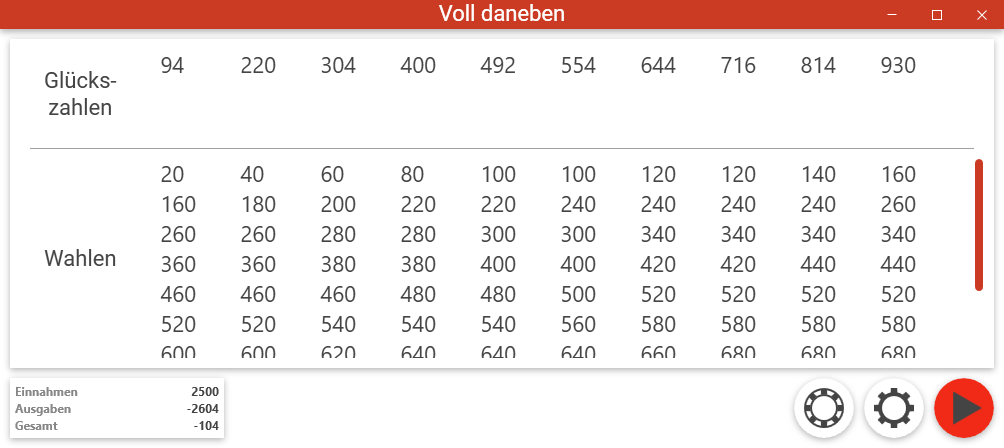
\includegraphics[scale=.5]{0}
\captionof{figure}{Greedy Solver ohne Optimierer}
\end{center}
\newpage
Lassen wir nun den Optimierer für 5 Iterationen laufen:\\
\begin{center}
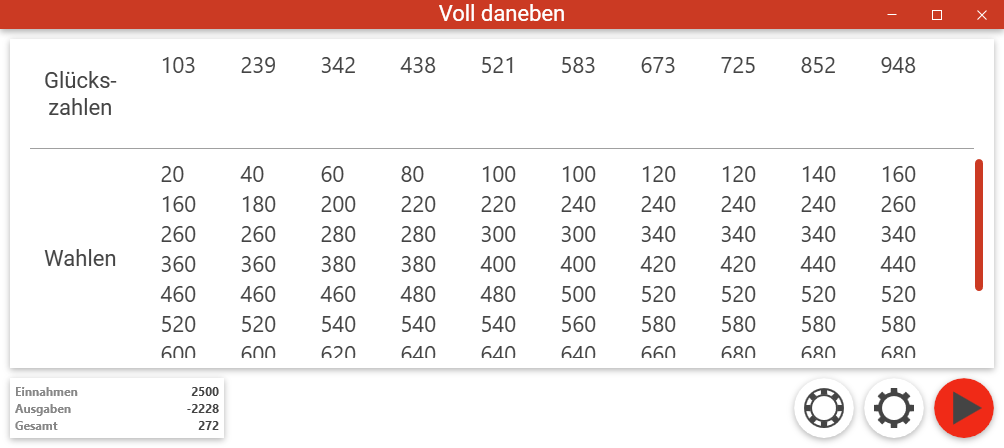
\includegraphics[scale=.5]{5}
\captionof{figure}{5 Iterationen}
\end{center}

\begin{center}
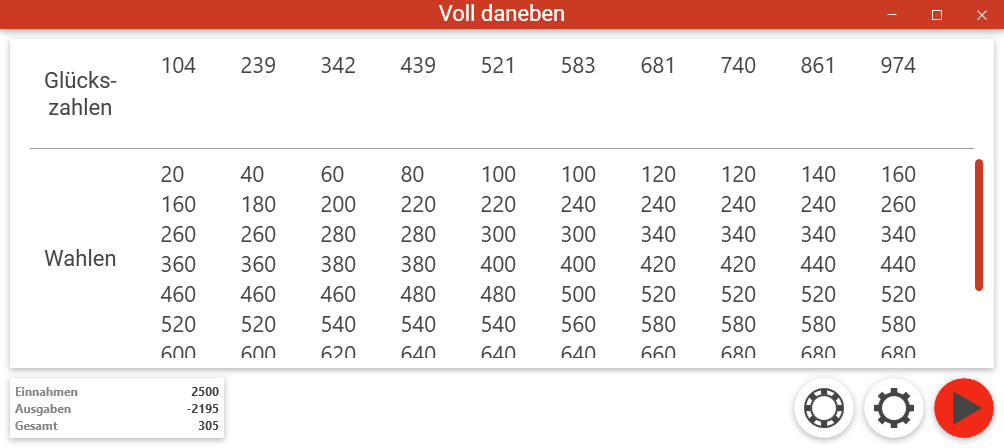
\includegraphics[scale=.5]{50}
\captionof{figure}{50 Iterationen}
\end{center}

Die Kosten haben sich also von 0 Iterationen zu 50 eindeutig stark verbessert. 
\subsection{Code}
In der Implementierung haben wir zunächst eine Methode $Cost(numbers,\;selected\_numbers)$ beschrieben. Diese ist folgendermaßen implementiert:
\begin{Csharp}
public static int Cost(int[] choices, int[] luckyNumbers) 
	=> choices.Sum(x => luckyNumbers.Min(y => Math.Abs(y - x)));
\end{Csharp}
Im Prinzip sucht der Algorithmus für jede Zahl $n$ in $numbers$ die Zahl $s$ in $selected\_numbers$ mit der geringsten absoluten Differenz $|n-s|$ und summiert alle diese Differenzen. Da für jedes Element in $numbers$ eine $Min$ Operation auf $length(selected\_numbers) = 10$ durchgeführt werden muss, ist die Komplexität $O(length(numbers)\cdot10) = O(length(numbers))$.\\
\newpage
Weiterhin wurde eine Methode beschrieben, die die Initialverteilung der $selected\_numbers$ bestimmt. Sie ist folgendermaßen implementiert:
\begin{Csharp}
private static double[] BasicSolver(int[] choices, int availablePoints)
{
    Array.Sort(choices = choices.Distinct().ToArray());

    return Enumerable
        .Range(0, availablePoints)
        .Select(x =>
            Enumerable.Range(
            	x * (int)Math.Floor((double)choices.Length / availablePoints), 
            	  (int)Math.Ceiling((double)choices.Length / availablePoints))
            .Average(y => choices[y]))
        .ToArray();
}
\end{Csharp}
Es hat sich durch Testen erwiesen, dass es optimal ist $numbers$ in 10 Gruppen aufzuteilen und von jeder den Durchschnitt zu bestimmen und diese Durchschnitte als zu optimierende $selected\_numbers$ zu betrachten.\\

Der Gradient-Descent Algorithmus:
\begin{Csharp}
public static double[] OptimizeSolution(int[] choices, double[] luckyNumbers,
	int start, int passes, int stride)
{
    if (passes > 0)
    {
        int availablePoints = luckyNumbers.Length;
        double min = choices.Min(), max = choices.Max();
        double[] costs =
        	Enumerable.Repeat(Cost(choices, luckyNumbers), availablePoints)
        	.ToArray();

        for (int pass = start; pass < passes + start; pass += stride)
        {
            double move = (max - min) / pass;

            for (int i = 0; i < availablePoints; i++)
            {
                double prevNumber = luckyNumbers[i];

                luckyNumbers[i] = Math.Max(min, prevNumber - move);
                double leftCost = Cost(choices, luckyNumbers);

                luckyNumbers[i] = Math.Min(max, prevNumber + move);
                double rightCost = Cost(choices, luckyNumbers);

                luckyNumbers[i] = prevNumber;

                if (leftCost < rightCost && leftCost < costs[i])
                {
                    luckyNumbers[i] = Math.Max(min, prevNumber - move);
                    costs[i] = leftCost;
                }
                else if(rightCost < costs[i])
                {
                    luckyNumbers[i] = Math.Min(max, prevNumber + move);
                    costs[i] = rightCost;
                }
            }
        }
    }

    return luckyNumbers.ToArray();
}
\end{Csharp}
besteht vereinfacht aus einer äußeren Schleife, die für jeden Optimierungsschritt wie im \textbf{Lösungsansatz} beschrieben n-mal durchläuft. Im inneren dieser Schleife befindet sich eine weitere Loop, die durch die $selected\_numbers$ iteriert und jede Zahl erhöht oder ansenkt je nach dem was die Kosten Funktion $Cost$ mehr senkt. 

\end{flushleft}
\end{document}